\section{Propósito y base del trabajo}

Nuestro proyecto se basa en un artículo de RapGenius, cliente del proveedor Heroku. En este artículo, RapGenius critica
el reciente cambio en la política de load-balancing de su proveedor, mostrando, con resultados de simulaciones corridas
en R, que ese cambio resulta en resultados pésimos. Según RapGenius, una empresa necesitaría
cincuenta veces más servidores corriendo la misma aplicación para alcanzar la misma disponibilidad con el nuevo modelo
de routing, muy sencillo, que la que permitía el antiguo modelo, que usaba un algoritmo más complicado.

\begin{figure}[h]
    \centering
    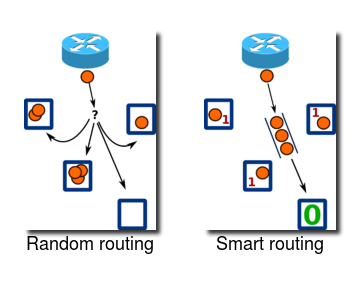
\includegraphics[height=200px]{random-smart.png}
    \caption{Los dos modelos presentados por RapGenius en su artículo}
    \label{fig:random+smart}
\end{figure}

El primer algoritmo, llamado ``Smart routing'', hace que cuando el \textit{router} recibe un pedido, lo manda a un servidor
desocupado. Si no hay, lo guarda en una cola. Cada vez que un servidor se desocupa, el pedido que llegó primero en la
cola va a este servidor. Entonces, en este modelo, no hay cola a nivel de servidores.

El segundo algoritmo se llama ``Random routing''. Es mucho más sencillo. El \textit{router} manda cada pedido que llega
a cualquier servidor. La única condición es que el servidor debe tener lugar en su cola. Si está lleno, el
\textit{router} intenta con otro servidor, hasta que encuentra un servidor o que alcanza un número máximo de intentos.
Si no logra encontrar un servidor con lugar en su cola, guarda el pedido en su propia cola.

En nuestro proyecto, el objetivo es comprobar los resultados de RapGenius y además verificar cuál podría ser el mejor
algoritmo. Por eso, estudiamos además del ``Smart routing'' y del ``Random routing'' otros dos algoritmos: el
``Round-robin routing'' y el ``Shortest queue routing'' (ver imagen \ref{fig:round_robin+shortest_queue}).

\begin{figure}[h]
    \centering
    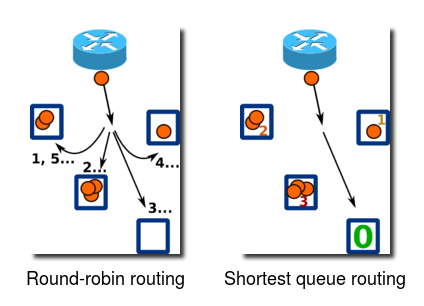
\includegraphics[height=200px]{round-robin--shortest-queue.png}
    \caption{Los otros dos modelos estudiados}
    \label{fig:round_robin+shortest_queue}
\end{figure}


El algoritmo de round-robin funciona de manera muy simple. El \textit{router} construye una lista circular\footnote{Una 
lista ``sin fin'' donde el elemento siguiente del último es el primero} de servidores y sabe a cual mandó el último pedido. 
Cuando recibe otro, lo manda al servidor siguiente en la lista, si ese tiene lugar en su cola. Si no, intenta con el
siguiente. Si ningún servidor tiene lugar, guarda el pedido en su propia cola.

Para finalizar, cuando usa el algoritmo de ``Shortest queue'', el \textit{router} manda cada pedido que llega al
servidor que tiene menos cola (o no cola) en este momento. Si hay más de un servidor con cola mínima, elige uno al
azar. Es el algoritmo más complicado de implementar, ya que requiere que el \textit{router} conozca el estado completo
de los servidores a cada momento.


